\section{Proposed Solution}
 
\subsection{Determination of Truss Inertia}

In order to accurately determine the truss inertia, the truss needs to be analyzed under actual operational conditions. 
According to speed-control equations for an armature-controlled DC motor, velocity is a function of a variety of either known or determinable system parameters ($A$, $K_m$, $K_b$, $K_t$, $R_a$, $B$, $J_{motor}$, $J_{magnet}$) and the unknown $J_{truss}$. 
In general, by solving for $J_{truss}$ and measuring velocity, the truss inertia can be calculated. 
To measure velocity, the truss was attached to the motor apparatus and operated at different set voltages while simultaneously recording encoder values for angular velocity. 
As will be discussed in the following section, the details of the truss inertia calculations involve time $t$ (before the system reaches final velocity), velocity at time $t$, final velocity $w_{fv}$, and input motor voltage $A$.

\subsection{Controller Design}

%TODO: Where percent overshoot and settling time equations come from.

The following steps were taken to find values for controller gains.

\begin{enumerate}
\item Find system transfer function with PD controller (shown in Equation \ref{eq:systf}).
\item Substitute actual values for system parameters. These parameters are listed in Table \ref{tbl:sysparams}.
\item Equate the coefficients of the characteristic equation to the prototype second order system such that an $\omega_n$ and $\zeta$ may be found.
	%TODO: show equation
\item Use the equation for percent overshoot to find $\zeta$. This is shown in Equation \ref{eq:po}. 
\item Use the equation for settling time to find $\omega_n$. This is shown in Equation \ref{eq:ts}.
\item Solve for $K_p$ and $K_d$.
	%TODO: Talk about more
\end{enumerate}

Since $\zeta < 0.69$, Equation \ref{eq:ts} may be used.
	%TODO: Move somewhere more appropriate
When solving a settling time of 0.6 seconds and maximum overshoot of 15\% was chosen.
	%TODO: Reference where this is discussed or discuss it here.
This resulted in desired controller gains of $K_p = 1.380778087$ and $ K_d = 0.1141262430 $.
A pole-zero plot for the system with these values may be seen in Figure \ref{fig:polezero}.

\begin{equation}
	\label{eq:systf}
	{\frac {\Theta_{out}}{\Theta_{in}}} = 
	{\frac 
		{\frac {\left( K_p +  K_d\,s \right)\,K_m\,K_s}{R\,J}}
		{s^{2} + {\frac {R\,B + K_m\,K_b + K_m\,K_s\,K_d}{R\,J}}\,s + {\frac {K_m\,K_s\,K_p}{R\,J}}}
	}
\end{equation}

\begin{equation}
	\label{eq:po}
	{\it PO}={{\rm e}^{-{\frac {\pi \,\zeta}{\sqrt {1-{\zeta}^{2}}}}}}
\end{equation}

\begin{equation}
	\label{eq:ts}
	{\it T_s} ={\frac {3.2}{\zeta\,\omega_n}}
\end{equation}

\begin{table}[htb]
	\centering
	\caption{System Parameters}
	\label{tbl:sysparams}
	\vspace{6pt}
	\footnotesize
	\begin{tabular}{cccc}
		\toprule
		Parameter & Name & Value & Source \\
		\midrule
		$K_b$ & Back EMF Constant & 0.02424 ${\frac {V}{rad/s}}$ & Motor Data Sheet \\
		$K_m$ & Motor Constant & 0.02424 ${\frac {N\,m}{A}}$ & Motor Data Sheet \\
		$R$ & Armature Resistance s& 2.23 $\Omega$ & Motor Data Sheet \\
		$B$ & Viscous Damping Friction & 0.00035 ${\frac {kg\,m^2}{s}}$ & Experimentally Determined \\
		$J$ & Total Inertia & 0.00141 $kg\,m^2$ & Experimentally Determined \\
		\bottomrule
	\end{tabular}
\end{table}

 \begin{figure}[ht]
    \centering
    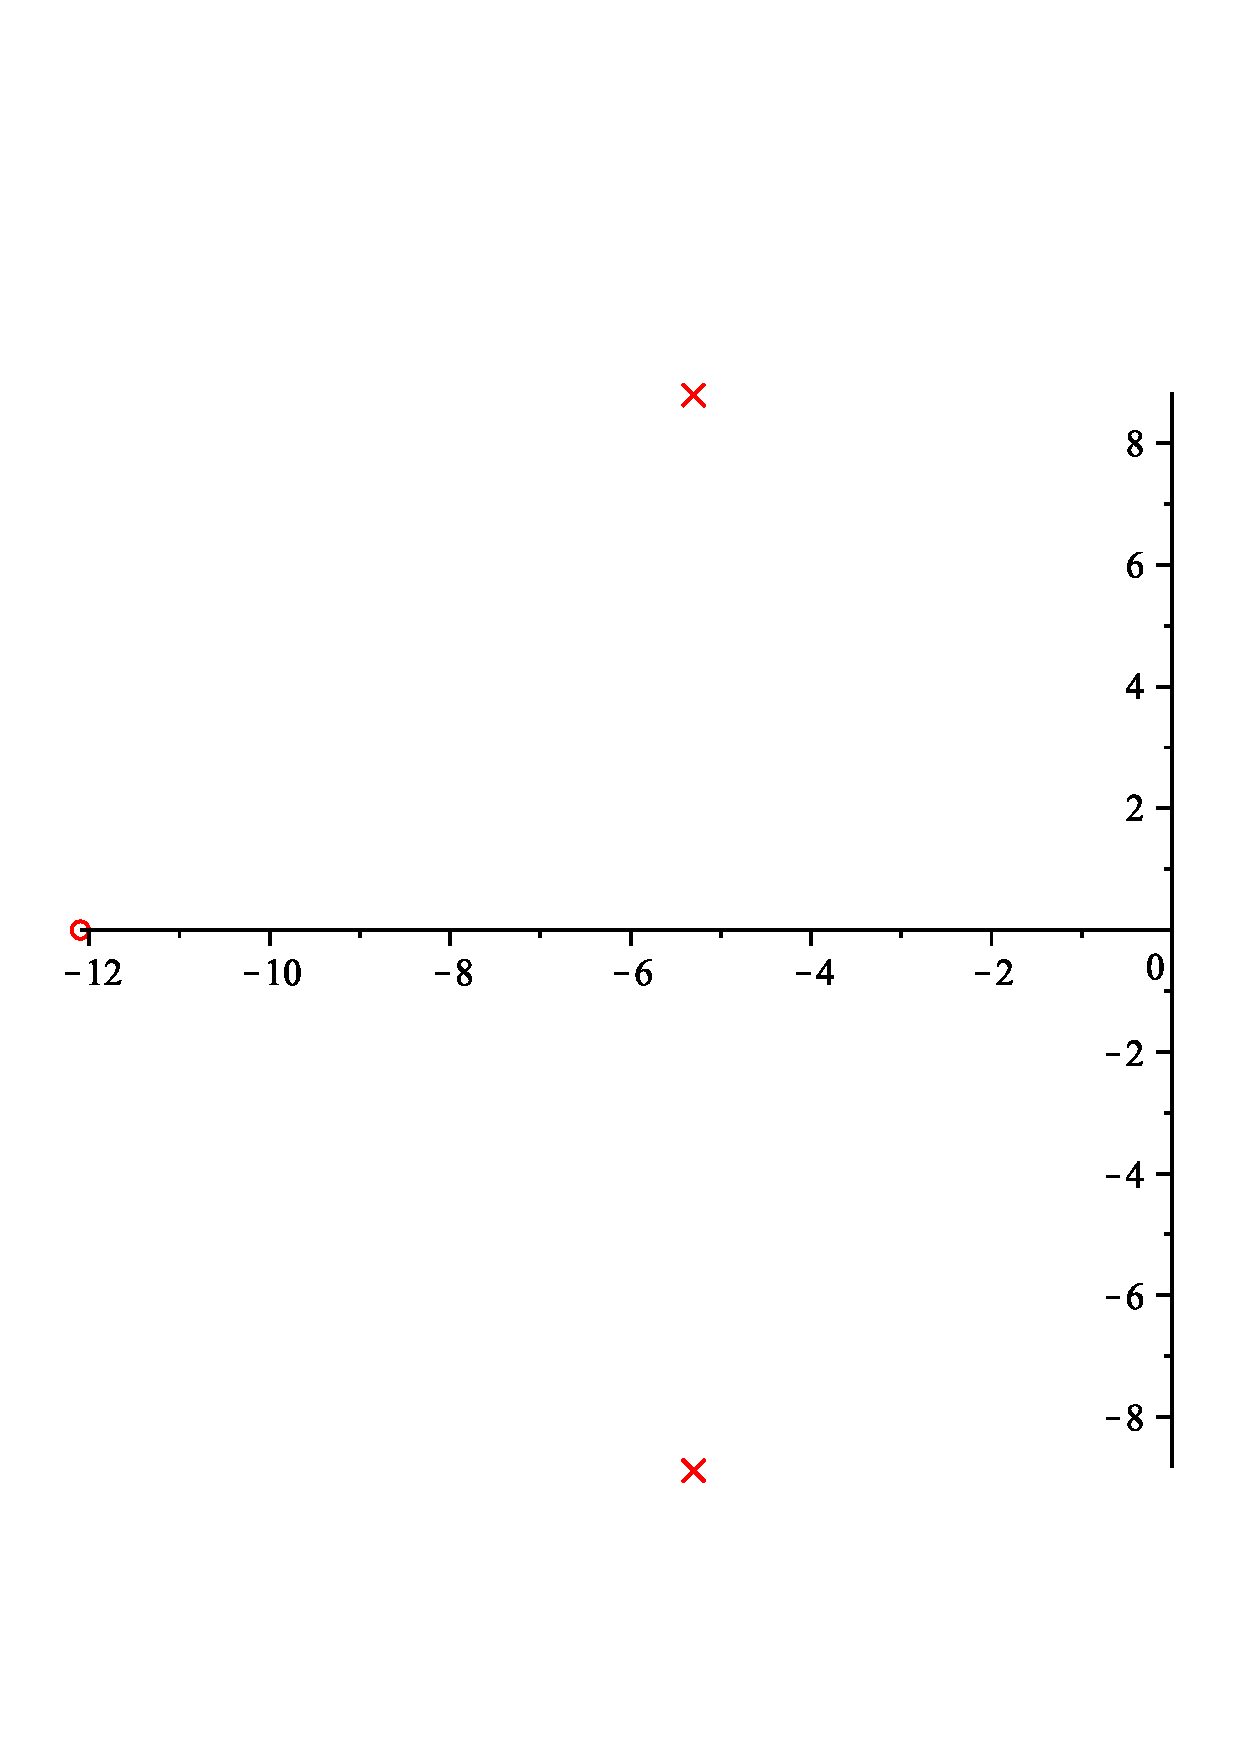
\includegraphics[width=.50\textwidth]{images/PoleZero.pdf}
    \caption{Pole-Zero Plot}
    \label{fig:polezero}
\end{figure}


\subsection{Simulation}

The ACSYS software system was used to simulate system behavior.
Correct system parameters were entered including gains to represent the gearbox.
A simulink block diagram for controller design may be seen in Figure \ref{fig:acsys}.

\begin{figure}[ht]
    \centering
    \includegraphics[width=.95\textwidth]{images/SimulinkBlockDiagram.PNG}
    \caption{ACSYS Control}
    \label{fig:acsys}
\end{figure}

\subsection{Amplifier Compensation}

Due to nonlinearities and difficulties controlling the amplifier with an analog input and on-board oscillator with peak detectors, the majority of the circuitry was bypassed.
Two digital to analog output of the computer controller were used and connected at the previous peak detector outputs.
Software PWM was then implemented; a simulink block model may be seen in Figure \ref{fig:swpwm}.
Two levels of feedback were also implemented correct for motor back EMF and simple error.

 \begin{figure}[ht]
    \centering
    \includegraphics[width=.99\textwidth]{images/swpwm.png}
    \caption{Simulink Software PWM With Velocity and Error Feedback Control}
    \label{fig:swpwm}
\end{figure}

